\documentclass[a4paper, 12pt]{article}

\def\languages{french, english}

%%%%%%%%%%%%%%%%%%% Libraries

%%%%%%%%%% Packages

\usepackage[
backend=biber,
style=numeric-comp,
sorting=none,
maxbibnames=99
]{biblatex}

\newgeometry{margin = 2.5cm}
\makeatletter
\begin{titlepage}
	\begin{minipage}[t][0.4125\textheight]{\textwidth}
		\begin{center}
		    \ifx\toptitle\undefined
    		    \ifx\logopath\undefined
    		    \else
    		    	\vfill
    			    \includegraphics[height=0.15\textheight]{\logopath}
    			\fi
    		\else
    		    \ifx\logopath\undefined
    		    \else
    			    \includegraphics[height=0.15\textheight]{\logopath}
    			\fi
    			\vfill
    			{\huge \textsc{\toptitle}}
			\fi
			\vfill
		\end{center}
	\end{minipage}
	\vfill
	\begin{minipage}{\textwidth}
		\hspace{0.5em}
		\begin{mdframed}[linewidth = 2pt, innertopmargin = 1em, innerbottommargin = 1em, leftline = false, rightline = false]
			\begin{center}
				{\huge \bfseries \@title}
			\end{center}
		\end{mdframed}
		\hspace{0.5em}
		\ifx\subtitle\undefined
		\else
		\begin{center}
			{\LARGE \subtitle}
		\end{center}
		\fi
	\end{minipage}
	\vfill
	\begin{minipage}[b][0.4125\textheight][t]{\textwidth}
			\vfill
			\ifx\rightauthor\undefined
			    \begin{center}
			        \ifx\authorhead\undefined
			        \else
		                {\large\it \authorhead\\[0.5em]}
		            \fi
			        {\large \@author}
			    \end{center}
			\else
			    \begin{minipage}[t]{0.5\textwidth}
			        \begin{flushleft}
			            \ifx\authorhead\undefined
			            \else
			                {\large\it \authorhead\\[0.5em]}
			            \fi
				        {\large \@author}
				    \end{flushleft}
				\end{minipage}
				\begin{minipage}[t]{0.5\textwidth}
				    \begin{flushright}
				        \ifx\rightauthorhead\undefined
			            \else
			                {\large\it \rightauthorhead\\[0.5em]}
			            \fi
				        {\large \rightauthor}
				    \end{flushright}
				\end{minipage}
			\fi
			\vfill
			\begin{center}
			    \ifx\context\undefined
			    \else
			        {\large \context \\[0.5em]}
			    \fi
			    {\large \@date}
			\end{center}
	\end{minipage}
\end{titlepage}
\makeatother
\restoregeometry
%%%%%%%%%% Packages

\usepackage{float}
\usepackage[skip=1em]{caption}

\usepackage{array}
\usepackage{multirow}
\usepackage{multicol}

%%%%%%%%%% Features

%%%%% Settings

\renewcommand{\arraystretch}{1.2}

%%%%% Commands

\newcommand\noskipcaption[1]{\caption{#1}\vspace{-1em}}
\newcommand\noskipcaptionstar[1]{\caption*{#1}\vspace{-1em}}

%%%%%%%%%% Packages

\usepackage{inconsolata}
\usepackage{listings}

%%%%%%%%%% Features

%%%%% Commands

\newcommand{\Nstyle}[1]{
    \lstdefinestyle{N#1}{
        style=#1,
        %%%%%
        numbers=left
    }
}

\newcommand{\tbFstyle}[1]{
    \lstdefinestyle{tbF#1}{
        style=#1,
        %%%%%
        frame=tb
    }
}

\newcommand{\Fstyle}[1]{
    \lstdefinestyle{F#1}{
        style=#1,
        %%%%%
        frame=single,
        framesep=0em,
        rulesep=0em,
        xleftmargin=0.75em,
        xrightmargin=0.75em,
        framexleftmargin=0.75em,
        framexrightmargin=0.75em,
        framextopmargin=0.5em,
        framexbottommargin=0.5em,
        %%%%%
        numbersep=1.25em
    }
}

\newcommand{\NtbFstyle}[1]{
    \tbFstyle{#1}
    \Nstyle{tbF#1}
}

\newcommand{\NFstyle}[1]{
    \Fstyle{#1}
    \lstdefinestyle{NF#1}{
        style=f#1,
        %%%%%
        xleftmargin=2.75em,
        framexleftmargin=2.75em,
        %%%%%
        numbers=left,
        numbersep=1em
    }
}

%%%%% Styles

\lstdefinestyle{default}{
    breaklines=true,
    breakatwhitespace=true,
    columns=fixed,
	extendedchars=true,
    upquote=true,
	tabsize=4,
    %%%%%
    framerule=0.66pt,
    captionpos=b,
	%%%%%
    basicstyle=\footnotesize\ttfamily,
    numberstyle=\footnotesize\ttfamily,
    showstringspaces=false
}
\Nstyle{default}
\NFstyle{default}
\NtbFstyle{default}

\lstdefinestyle{monokai}{
    style=Fdefault,
    %%%%%
    backgroundcolor=\color[HTML]{272822},
    framerule=0em,
    %%%%%
    basicstyle=\footnotesize\ttfamily\color[HTML]{f8f8f2},
    numberstyle=\footnotesize\ttfamily\color[HTML]{272822},
    commentstyle=\color[HTML]{75715e},
    keywordstyle=[1]{\color[HTML]{f92672}},
    keywordstyle=[2]{\color[HTML]{A6E22E}},
    keywordstyle=[3]{\color[HTML]{ae81ff}},
    stringstyle=\color[HTML]{e6db74},
    %%%%%
    % otherkeywords={!,.,+,-,*,/,=,<,>,^,|,\&,OR,AND}
}

\lstdefinestyle{Nmonokai}{
    style=monokai,
    %%%%%
    xleftmargin=2.75em,
    framexleftmargin=2.75em,
    %%%%%
    numbers=left,
    numberstyle=\footnotesize\ttfamily\color[HTML]{f8f8f2},
    numbersep=1em
}

\lstdefinestyle{c}{
    language=C,
    style=default,
    %%%%%
    commentstyle=\color[HTML]{228B22},
    keywordstyle=\color[HTML]{0000FF},
    stringstyle=\color[HTML]{A020F0},
    emphstyle=\color[HTML]{0000FF},
    %%%%%
    emph={}
}

\lstdefinestyle{cpp}{
    language=C++,
    style=default,
    %%%%%
    commentstyle=\color[HTML]{228B22},
    keywordstyle=\color[HTML]{0000FF},
    stringstyle=\color[HTML]{A020F0},
    emphstyle=\color[HTML]{0000FF},
    %%%%%
    emph={std}
}

\lstdefinestyle{matlab}{
    language=matlab,
    style=default,
    %%%%%
    basicstyle=\footnotesize\fontfamily{pcr}\selectfont,
    numberstyle=\footnotesize\fontfamily{pcr}\selectfont,
    commentstyle=\color[HTML]{228B22},
    keywordstyle=\color[HTML]{0000FF},
    stringstyle=\color[HTML]{A020F0},
    emphstyle=\color[HTML]{0000FF},
    %%%%%
    emph={clearvars}
}

\lstdefinestyle{python}{
    language=python,
    style=default,
    %%%%%
    commentstyle=\color[RGB]{221,0,0},
    keywordstyle=[1]{\color[RGB]{255,119,0}},
    keywordstyle=[2]{\color[RGB]{144,0,144}},
    stringstyle=\color[RGB]{0,170,0},
    emphstyle=\color[RGB]{255,119,0},
    %%%%%
    emph={}
}

\lstdefinestyle{java}{
    language=java,
    style=default,
    %%%%%
    commentstyle=\color[HTML]{228B22},
    keywordstyle=\color[HTML]{0000FF},
    stringstyle=\color[HTML]{A020F0},
    emphstyle=\color[HTML]{0000FF},
    %%%%%
    emph={}
}

%%%%%%%%%% Packages

\usepackage{amsmath}
\usepackage{amssymb}
\usepackage{bm}
\usepackage{esint}
\usepackage[makeroom]{cancel}

%%%%%%%%%% Features

%%%%% Macros

\newcommand{\rbk}[1]{\left(#1\right)}
\newcommand{\cbk}[1]{\left\{#1\right\}}
\newcommand{\sbk}[1]{\left[#1\right]}
\newcommand{\abs}[1]{\left|#1\right|}
\newcommand{\norm}[1]{\left\|#1\right\|}

\newcommand{\fact}[1]{#1!}
\newcommand{\e}[1]{\mathbf{e}_{#1}}
\newcommand{\deriv}{\mathrm{d}}
\DeclareMathOperator{\tr}{tr}

\def\Rl{\mathbb{R}}
\def\Cx{\mathbb{C}}
\def\Na{\mathbb{N}}
\def\Zi{\mathbb{Z}}

%%%%%%%%%% Packages

\usepackage{amsthm}
\usepackage{thmtools}

%%%%%%%%%% Features

%%%%% Settings

\makeatletter
\define@key{thmdef}{mdthm}[{}]{
	\thmt@trytwice{\def\thmt@theoremdefiner{\mdtheorem[#1]}}{}}
\makeatother

\begingroup
\makeatletter
\@for\theoremstyle:=plain,definition,remark\do{
	\expandafter\g@addto@macro\csname th@\theoremstyle\endcsname{
		\addtolength\thm@preskip\parskip
	}
}
\endgroup

\renewcommand{\qedsymbol}{$\blacksquare$}

% language

\ifx\lgthm\undefined
	\def\lgthm{Theorem}
	\def\lgprf{Proof}
	\def\lglem{Lemma}
	\def\lgprop{Proposition}
	\def\lgdefn{Definition}
	\def\lghyp{Hypothesis}
	\def\lgmeth{Method}
	\def\lgquest{Question}
	\def\lgansw{Answer}
	\def\lgexpl{Example}
	\def\lgrmk{Remark}
	\def\lgnote{Note}
	\def\lgtip{Tip}
\fi

%%%%% Commands

\newcommand\qedadd{\pushQED{\qed}\popQED}

%%%%% Environments

\theoremstyle{plain}
\newtheorem{thm}{\lgthm}
\newtheorem{lem}[thm]{\lglem}
\newtheorem{prop}[thm]{\lgprop}

\theoremstyle{definition}
\newtheorem{defn}{\lgdefn}
\newtheorem{hyp}{\lghyp}
\newtheorem{meth}{\lgmeth}
\newtheorem{quest}{\lgquest}

\theoremstyle{remark}
\newtheorem{answ}{\lgansw}[quest]
\newtheorem{expl}{\lgexpl}
\newtheorem*{rmk}{\lgrmk}
\newtheorem*{note}{\lgnote}
\newtheorem*{tip}{\lgtip}

% framed

\mdfdefinestyle{thicc}{
	nobreak=true,
	skipabove=\topskip,
	skipbelow=\topskip,
	innerleftmargin=0.5em,
	innerrightmargin=0.5em,
	innerbottommargin=0.5em,
	innertopmargin=0.5em,
	linewidth=0.25em,
	roundcorner=0.15em,
	linecolor=black!10,
	frametitlebackgroundcolor=black!10,
	theoremseparator={.}
}

\declaretheorem[mdthm={style=thicc, linecolor=red!20, frametitlebackgroundcolor=red!20}, sibling=thm, name=\lgthm]{framedthm}
\declaretheorem[mdthm={style=thicc, linecolor=red!20, frametitlebackgroundcolor=red!20}, sibling=thm, name=\lglem]{framedlem}
\declaretheorem[mdthm={style=thicc, linecolor=blue!20, frametitlebackgroundcolor=blue!20}, sibling=thm, name=\lgprop]{framedprop}
\declaretheorem[mdthm={style=thicc, nobreak=false}, parent=thm, name=\lgprf]{framedprf}

\declaretheorem[mdthm={style=thicc, linecolor=black!20!green!20, frametitlebackgroundcolor=black!20!green!20}, sibling=defn, name=\lgdefn]{frameddefn}
\declaretheorem[mdthm={style=thicc, linecolor=blue!20, frametitlebackgroundcolor=blue!20}, sibling=hyp, name=\lghyp]{framedhyp}
\declaretheorem[mdthm={style=thicc}, name=\lgmeth]{framedmeth}
\declaretheorem[mdthm={style=thicc, linecolor=orange!20, frametitlebackgroundcolor=orange!20}, sibling=quest, name=\lgquest]{framedquest}

\declaretheorem[mdthm={style=thicc, nobreak=false}, sibling=answ, name=\lgansw]{framedansw}
\declaretheorem[mdthm={style=thicc, nobreak=false}, sibling=expl, name=\lgexpl]{framedexpl}

%%%%%%%%%% Packages

\usepackage{siunitx}

%%%%%%%%%% Features

%%%%% Settings

\ifx\decimalsign\undefined
\else
    \sisetup{output-decimal-marker = \decimalsign}
\fi


%%%%%%%%%%%%%%%%%%% Titlepage

\def\logopath{resources/pdf/logo-uliege.pdf}
\def\toptitle{University of Liège}
\title{Active mass damper}
\def\subtitle{Linear control systems}
%\def\authorhead{Author}
\author{
    Bastien \textsc{Hoffmann} (20161283)\\
    Maxime \textsc{Meurisse} (20161278)\\
    Valentin \textsc{Vermeylen} (20162864)\\
}
%\def\rightauthorhead{}
%\def\rightauthor{}
\def\context{Master in Civil Engineering}
\date{Academic year 2019-2020}

%%%%%%%%%%%%%%%%%%% Options

\fancyhead[R]{}
\addbibresource{references.bib}
\defbibheading{bibliography}[\refname]{}

%%%%%%%%%%%%%%%%%%% Document

\begin{document}
    % ----- Titlepage ----- %
    \newgeometry{margin = 2.5cm}
\makeatletter
\begin{titlepage}
	\begin{minipage}[t][0.4125\textheight]{\textwidth}
		\begin{center}
		    \ifx\toptitle\undefined
    		    \ifx\logopath\undefined
    		    \else
    		    	\vfill
    			    \includegraphics[height=0.15\textheight]{\logopath}
    			\fi
    		\else
    		    \ifx\logopath\undefined
    		    \else
    			    \includegraphics[height=0.15\textheight]{\logopath}
    			\fi
    			\vfill
    			{\huge \textsc{\toptitle}}
			\fi
			\vfill
		\end{center}
	\end{minipage}
	\vfill
	\begin{minipage}{\textwidth}
		\hspace{0.5em}
		\begin{mdframed}[linewidth = 2pt, innertopmargin = 1em, innerbottommargin = 1em, leftline = false, rightline = false]
			\begin{center}
				{\huge \bfseries \@title}
			\end{center}
		\end{mdframed}
		\hspace{0.5em}
		\ifx\subtitle\undefined
		\else
		\begin{center}
			{\LARGE \subtitle}
		\end{center}
		\fi
	\end{minipage}
	\vfill
	\begin{minipage}[b][0.4125\textheight][t]{\textwidth}
			\vfill
			\ifx\rightauthor\undefined
			    \begin{center}
			        \ifx\authorhead\undefined
			        \else
		                {\large\it \authorhead\\[0.5em]}
		            \fi
			        {\large \@author}
			    \end{center}
			\else
			    \begin{minipage}[t]{0.5\textwidth}
			        \begin{flushleft}
			            \ifx\authorhead\undefined
			            \else
			                {\large\it \authorhead\\[0.5em]}
			            \fi
				        {\large \@author}
				    \end{flushleft}
				\end{minipage}
				\begin{minipage}[t]{0.5\textwidth}
				    \begin{flushright}
				        \ifx\rightauthorhead\undefined
			            \else
			                {\large\it \rightauthorhead\\[0.5em]}
			            \fi
				        {\large \rightauthor}
				    \end{flushright}
				\end{minipage}
			\fi
			\vfill
			\begin{center}
			    \ifx\context\undefined
			    \else
			        {\large \context \\[0.5em]}
			    \fi
			    {\large \@date}
			\end{center}
	\end{minipage}
\end{titlepage}
\makeatother
\restoregeometry
    
    % ----- Table of contents ----- %
    \romantableofcontents
    
    % ----- Homework 1 : Motivation and control problem ----- %
    \section{Motivation and control problem}
    \subsection{Context}
The current engineering prowesses allow us to construct buildings higher and higher. These constructions are subject to various disturbances (mainly wind, but also earthquakes) that make them oscillate. They turn into giant pendulum and swing from left to right, sometimes moving several meters at the top !\cite{YouTube_minutephysics}\par
To reduce these oscillations, we use a passive system, called {\it tuned mass damper}, which consists of concealing a tuned and harmonic oscillator at the top of the tower. It is coupled to its movement and oscillates in phase opposition to recover the kinetic energy of the tower and thus reduces the oscillations.\cite{Wikipedia_amortisseur_tmd}\par
An active version of this system exists : the {\it active mass damper}. It consists of the same principle as the tuned mass damper but it is equipped with sensors and actuators to measure the oscillations of its environment and, via an algorithm, generate a movement for the mass that reduce, or totally remove, these oscillations.\cite{sciencedirect_amd}\par
Our study field focuses on the active mass damper systems used to reduce the oscillations caused by the {\bf wind} on {\bf tall} buildings. More specifically, we will focus on a simplified model : a block linked to a spring (to simulate the oscillations of the building) and a smaller moving mass placed over it that stabilises the system.

    \subsection{Control problem diagram}
The diagram of our control problem is shown in figure \ref{fig:diagram}.
\begin{figure}[!ht]
    \centering
    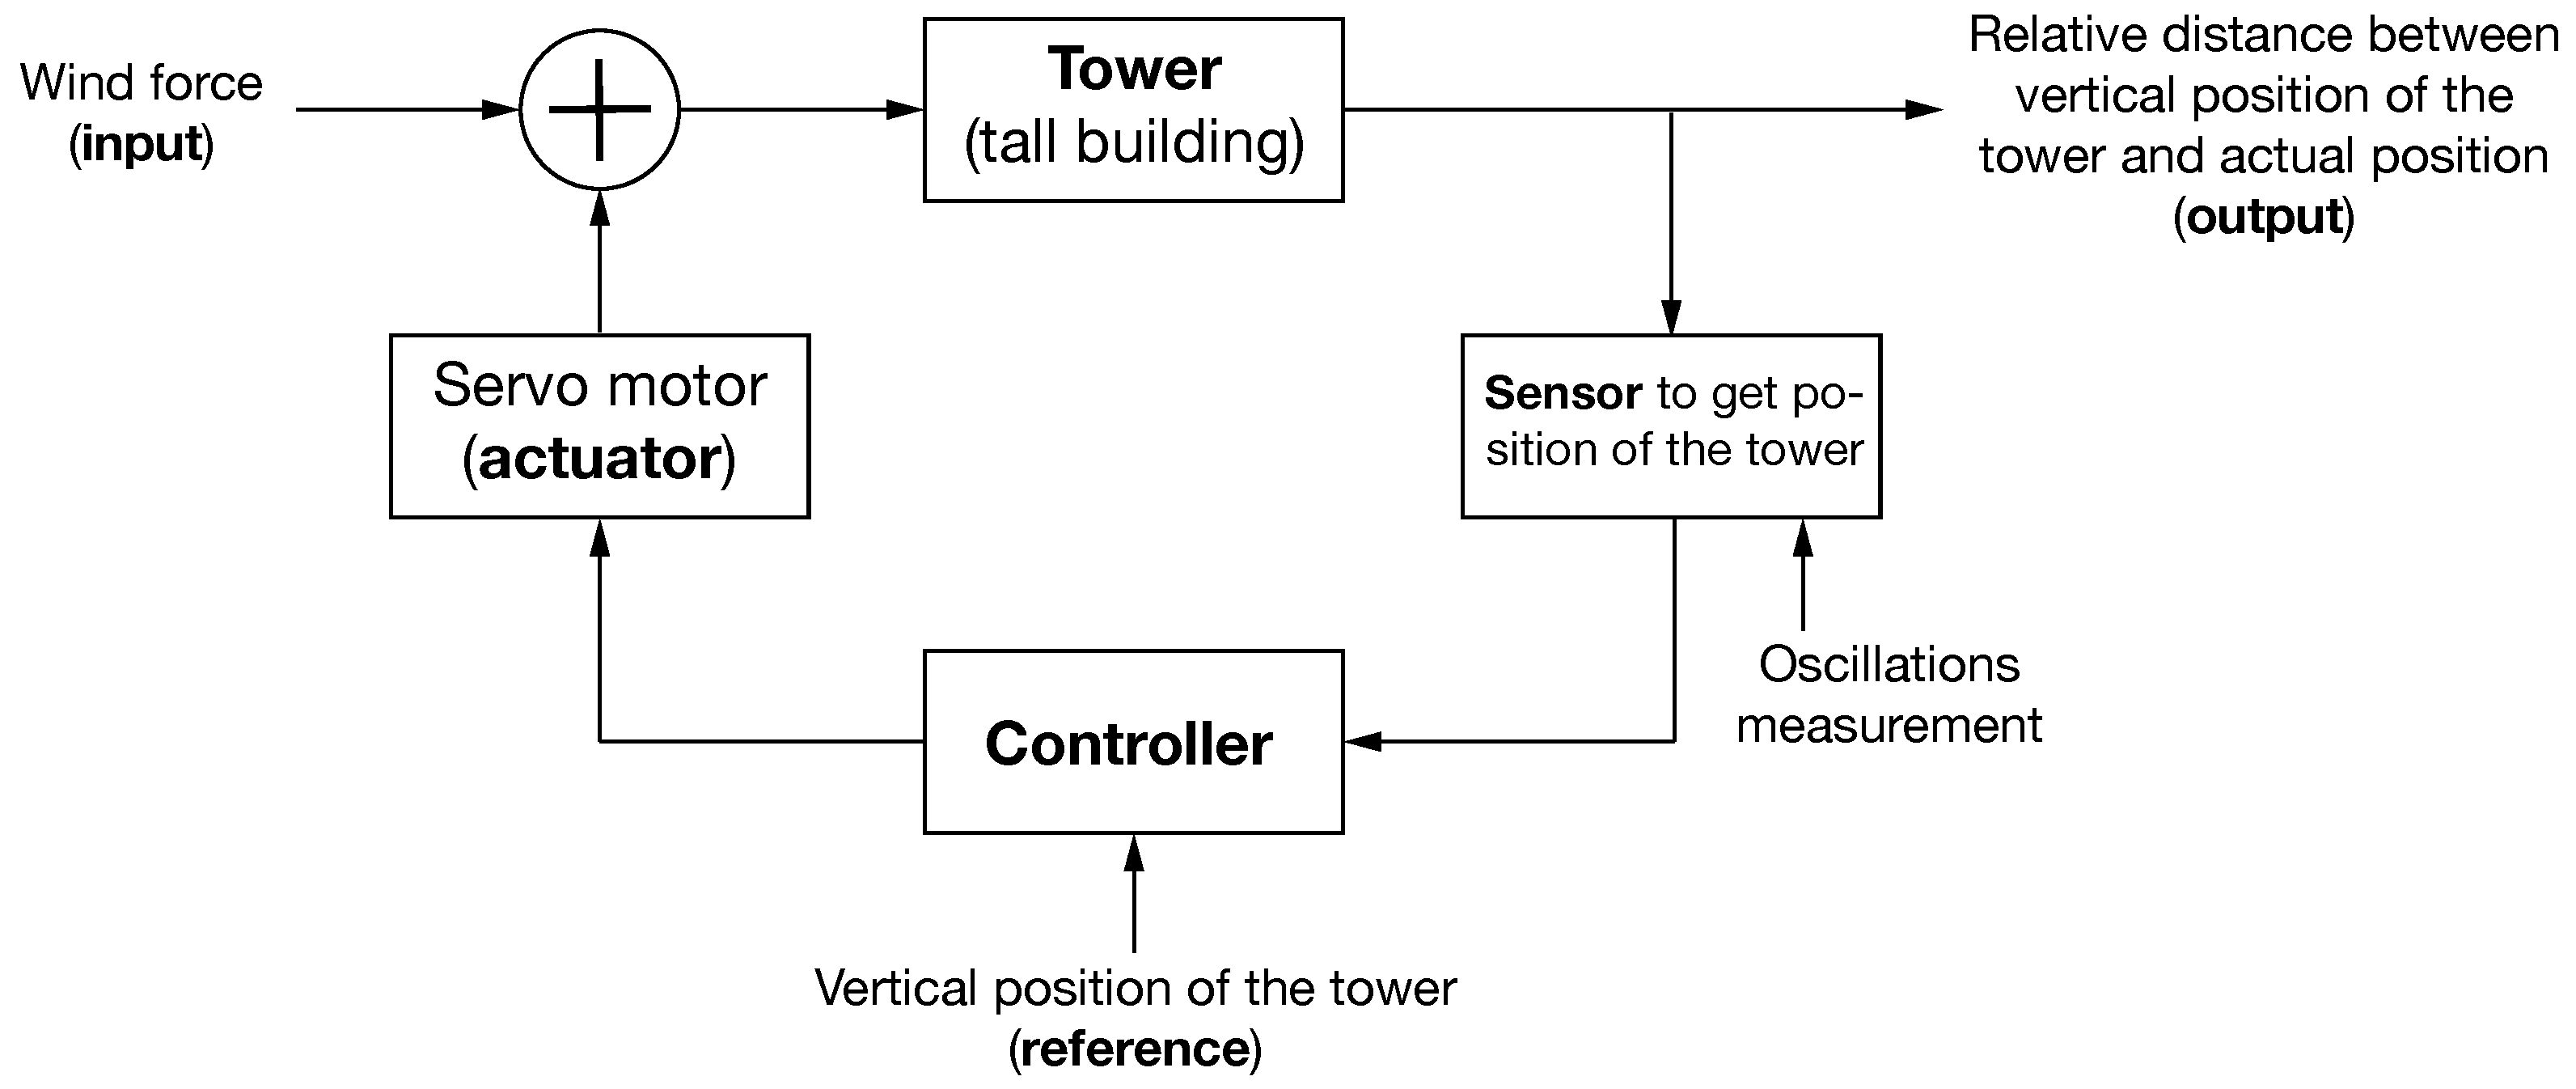
\includegraphics[width=1\textwidth]{resources/pdf/diagram.pdf}
    \caption{Control problem diagram of the active mass damper for tall buildings}
    \label{fig:diagram}
\end{figure}

    \subsection{Control problem description}
\begin{itemize}
    \item {\bf Utility of the controller} : the controller (the algorithm) allows the system (the tower) to be active, {\it i.e.} to measure the oscillations to which it is subjected and to cancel it. Thanks to a servo-motor connected to the controller, the mass can move and reduce, or even eliminate totally, the oscillations.
    \item {\bf System to be controlled} : the tower (and the position of the tower is the signal)
    \item {\bf Inputs of the system} : wind forces acting on the tower (uncontrollable) and on the moving mass (controllable).
    \item {\bf Outputs of the system} : the relative distance between the vertical position and the displacement of the tower.
    \item {\bf Reference} : the vertical position of the tower.
    \item {\bf Actuators} : servo-motor to move the mass that reduces the oscillations.
    \item {\bf Constraints and limitations} : to simplify our system, we consider a tower \SI{500}{\meter} high, perfectly vertical when it undergoes no disturbance. The only disturbance on this tower is the strength of the wind. The wind, ranging from a few tens of \SI{}{\kilo\meter/\hour} to a hundred \SI{}{\kilo\meter/\hour}, can swing the tower from a few centimetres to several meters.
\end{itemize}

    
    % ----- Homework 2 : Open loop system ----- %
    \section{Open loop system}
    \subsection{Detailed schematic of the open loop system}
The detailed schematic of the open loop studied system is shown in figure \ref{fig:detailed_schematic}.
\begin{figure}[H]
    \centering
    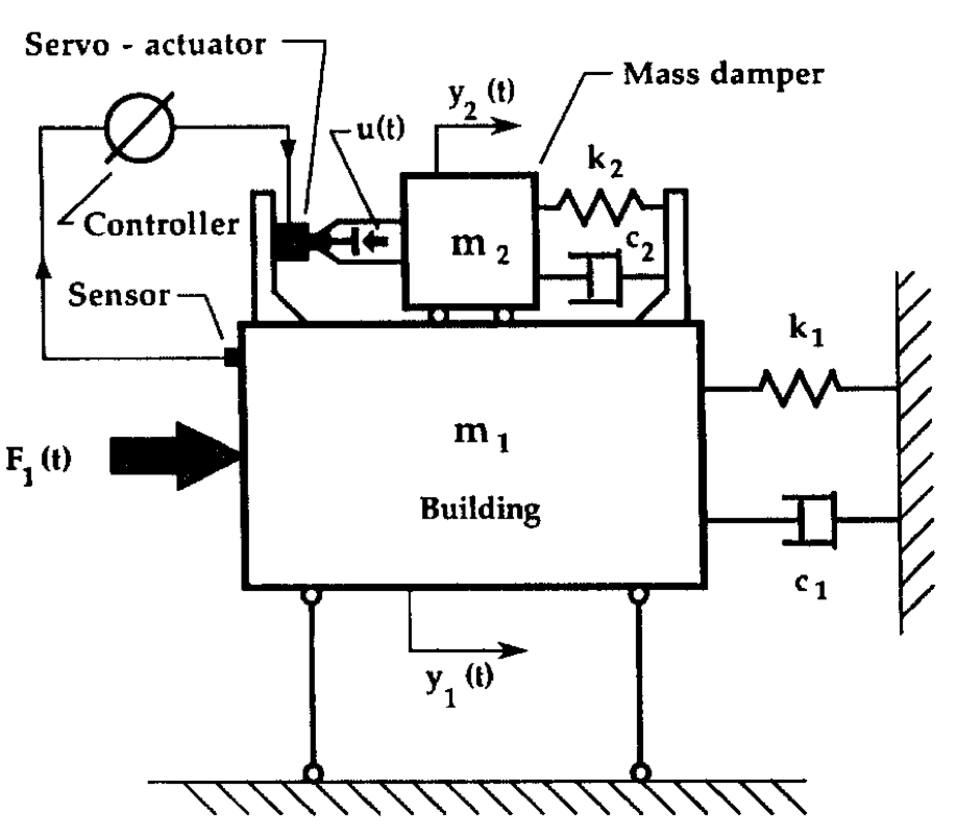
\includegraphics[width=0.7\textwidth]{resources/pdf/schema.pdf}
    \caption{Detailed schematic of the open loop studied system \cite{science_direct}}
    \label{fig:detailed_schematic}
\end{figure}
The building is represented by the mass $m_1$ and its oscillation motion is simulated by the spring $k_1$ and the damper $c_1$.\par
The mass damper is represented by the mass $m_2$ and its movement is simulated by the spring $k_2$ and the damper $c_2$.\par
The force $F_1(t)$ represents the wind force (uncontrollable) on the building.\par
The force $u(t)$ represents the force applied on the mass damper by the controller (controllable).\par
We are studying, at first, our system without a control mechanism. Our controllable input $u(t)$ will therefore be \num{0} for all our simulations in this section.

    \subsection{Constraints, assumptions, limitations}
To model and study the system, we defined a series of constraints, assumptions and limitations, presented in table \ref{tab:constraints_assumptions_limitations}.\par
\begin{table}[H]
    \centering
    \begin{tabular}{|l|c|}
        \hline
        \multirow{2}{*}{{\bf Building}} & height of \SI{250}{\meter}, width of \SI{40}{\meter}\\ & movement along a single axis (horizontal)\\\hline
        {\bf Mass} & no friction between $m_1$ and $m_2$\\ \hline
    \end{tabular}
    \caption{Constraints, assumptions and limitations of the system.}
    \label{tab:constraints_assumptions_limitations}
\end{table}

    \subsection{State-space representation}
In the following representation, all the $y$ in the diagram have been replaced by $d$.\par
Input vector $U$ and state vector $X$ are given by :
$$
U = \begin{pmatrix}
    F_1 \\
    u
\end{pmatrix}
\hspace{3cm}
X = \begin{pmatrix}
    d_1 \\
    \dot d_1 \\
    d_2 \\ 
    \dot d_2 \\
\end{pmatrix}
$$

% Inputs
\subsubsection{Inputs}
\begin{itemize}
    \item $F_1(t)$, the force of the wind (uncontrollable).
    \item $u(t)$, the force applied on the mass damper (controllable).
\end{itemize}
Our sensor is a measurement of the horizontal position of the top of the building relatively to the vertical position $d_1 = 0$.\par
Our actuator provides a force on the mass of the dampener, sets it in motion.

% Outputs
\subsubsection{Outputs}
$y = d_1(t)$ the relative position of the building with respect to the vertical position.

% States
\subsubsection{States}
\begin{itemize}
    \item $x_1 = d_1$, as described above.
    \item $x_2 = \dot d_1$, the speed of the building.
    \item $x_3 = d_2$, the relative displacement of the mass damper.
    \item $x_4 = \dot d_2$, the speed of the mass damper.
\end{itemize}

% Output law
\subsubsection{Output law}
The output is one of the states : $y = x_1$.

% Input law
\subsubsection{Input law}
The input law is given by \cite{sciencedirect_amd_2} :
$$
\begin{cases}
    m_{1}\ddot{d}_{1} + c_{1}\dot{d}_{1} + k_{1}d_{1} = c_{2}\dot{z} + k_{2}z + F_{1}(t) - u(t)\\
    m_{2}\ddot{z} + c_{2}\dot{z} + k_{2}z = -m_{2}\ddot{d}_{1} + u(t)
\end{cases}
$$
with $z = d_2 - d_1$.\par
The system is \textbf{linear}. We can easily derive the ABCD matrices.
$$
A = \begin{pmatrix}
    0 & 1 & 0 & 0 \\
    \frac{-k_1-k_2}{m_1} & \frac{-c_2-c_1}{m_1} & \frac{k_2}{m_1} & \frac{c_2}{m_1} \\
    0 & 0 & 0 & 1 \\ 
    \frac{k_2}{m_2} & \frac{c_2}{m_2} & \frac{-k_2}{m_2} & \frac{-c_2}{m_2}\\
\end{pmatrix}
\quad
B = \begin{pmatrix}
    0 & 0\\
    \frac{1}{m_1} & -\frac{1}{m_1}\\
    0 & 0\\
    0 & \frac{1}{m_2}\\
\end{pmatrix}
$$
$$
C = \begin{pmatrix}
    1 & 0 & 0 & 0\\
\end{pmatrix}
\quad
D = \begin{pmatrix}
    0 & 0\\
\end{pmatrix}
$$

    \subsection{System simulations without controller}
To simulate the system (without control mechanism), we choose a series of numerical values, presented in table \ref{tab:numerical_values}\footnote{We would like to thank Professor Denoël for discussing these values with us.}.
\begin{table}[H]
    \centering
    \begin{tabular}{|l|c|c|}
        \hline
        {\bf Mass} & $m_1 = \SI{1e8}{\kilogram}$ & $m_2 = \SI{1e3}{\kilogram}$\\ \hline
        {\bf Spring} & $k_1 \approx \SI{4e9}{\newton/\meter}$ & $k_2 = \SI{e5}{\newton/\meter}$\\ \hline
        {\bf Damper} & $c_1 \approx \SI{1.3e7}{\newton\second/\meter}$ & $c_2 = \SI{e4}{\newton\second/\meter}$\\ \hline
        {\bf Wind} & \multicolumn{2}{c|}{$F_{max} = \SI{7.35e6}{\newton}$}\\ \hline
    \end{tabular}
    \caption{Numerical values of the system}
    \label{tab:numerical_values}
\end{table}
For the strength of the wind, we considered 2 cases (in newton) :
\begin{align*}
    F_1 &= F_{max}\quad\forall t & \text{Constant wind force}\\
    F_1(t) &= F_{max}\sin(2\pi t) & \text{Sinusoidal wind force}
\end{align*}
The stiffness and viscosity values for the building were obtained using the formulas :
\begin{align*}
    k_1 &= (2\pi f)^2m_1\\
    c_1 &= 2m_1(2\pi f)0.01
\end{align*}
where $f = \SI{1}{\hertz}$ is the natural frequency associated with the mass of the building.\par
The maximum wind force, on the other hand, was approximated by
\begin{equation*}
    F_{max} = \frac{1}{2}\rho v^2A
\end{equation*}
with
\begin{itemize}
    \item $\rho \approx \SI{1.2}{\kilogram/\meter\cubed}$, the air density;
    \item $v = \SI{35}{\meter/\second}$, the wind speed;
    \item $A = 250\times 40 = \SI{10000}{\meter\squared}$, the area of one side of the building.
\end{itemize}
\subsubsection{Simulation results}
\begin{figure}[H]
    \centering
    \begin{subfigure}{0.495\textwidth}
        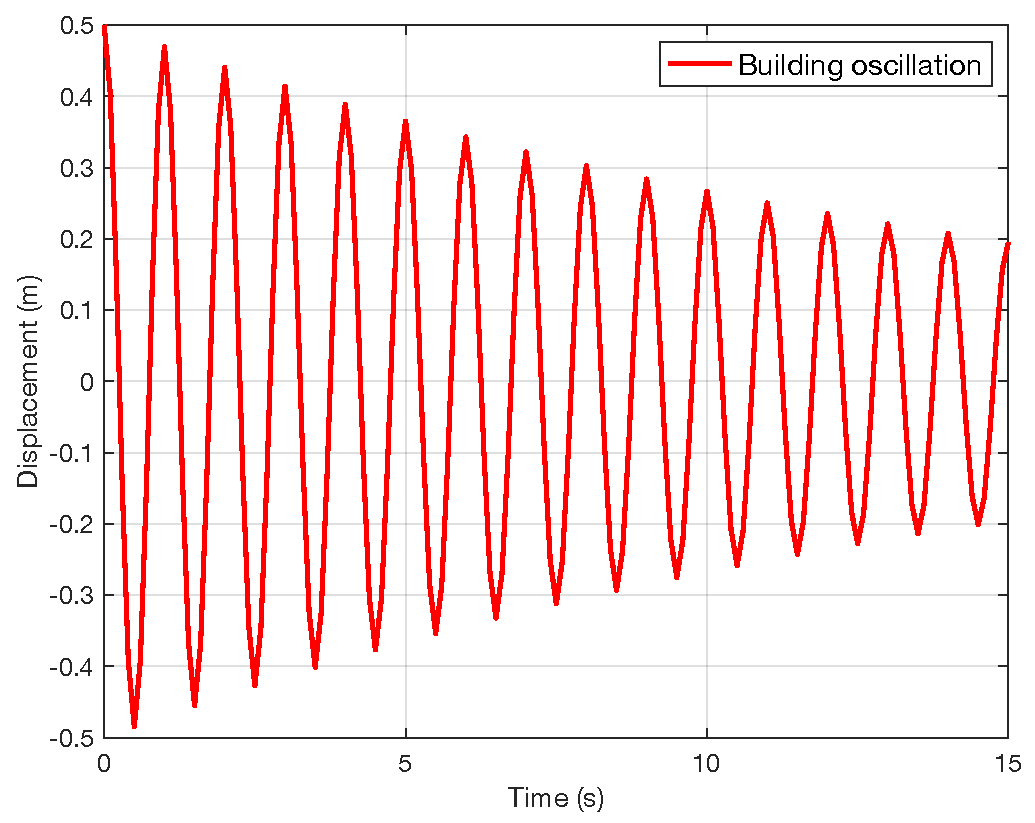
\includegraphics[width=\textwidth]{resources/pdf/initial.pdf}
        \caption{Initial conditions}
        \label{fig:q4.initial}
    \end{subfigure}
    \begin{subfigure}{0.495\textwidth}
        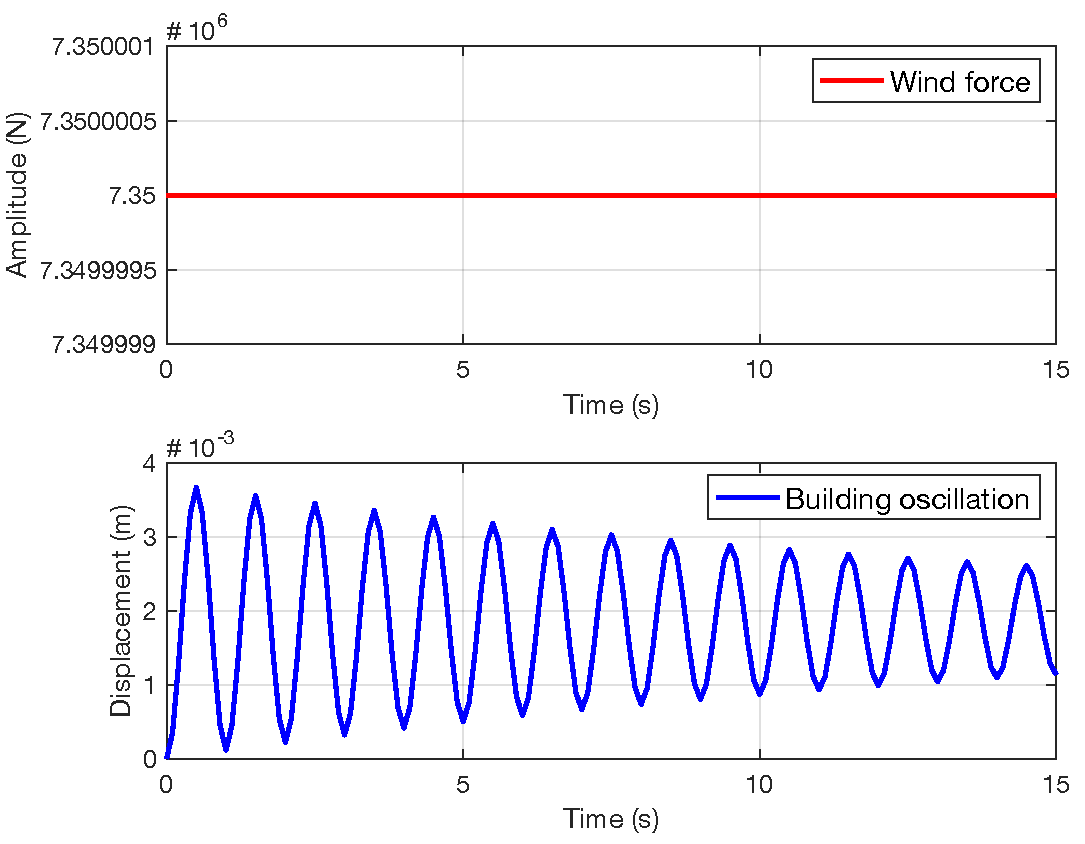
\includegraphics[width=\textwidth]{resources/pdf/constant.pdf}
        \caption{Constant wind force}
        \label{fig:q4.constant}
    \end{subfigure}
    \begin{subfigure}{0.495\textwidth}
        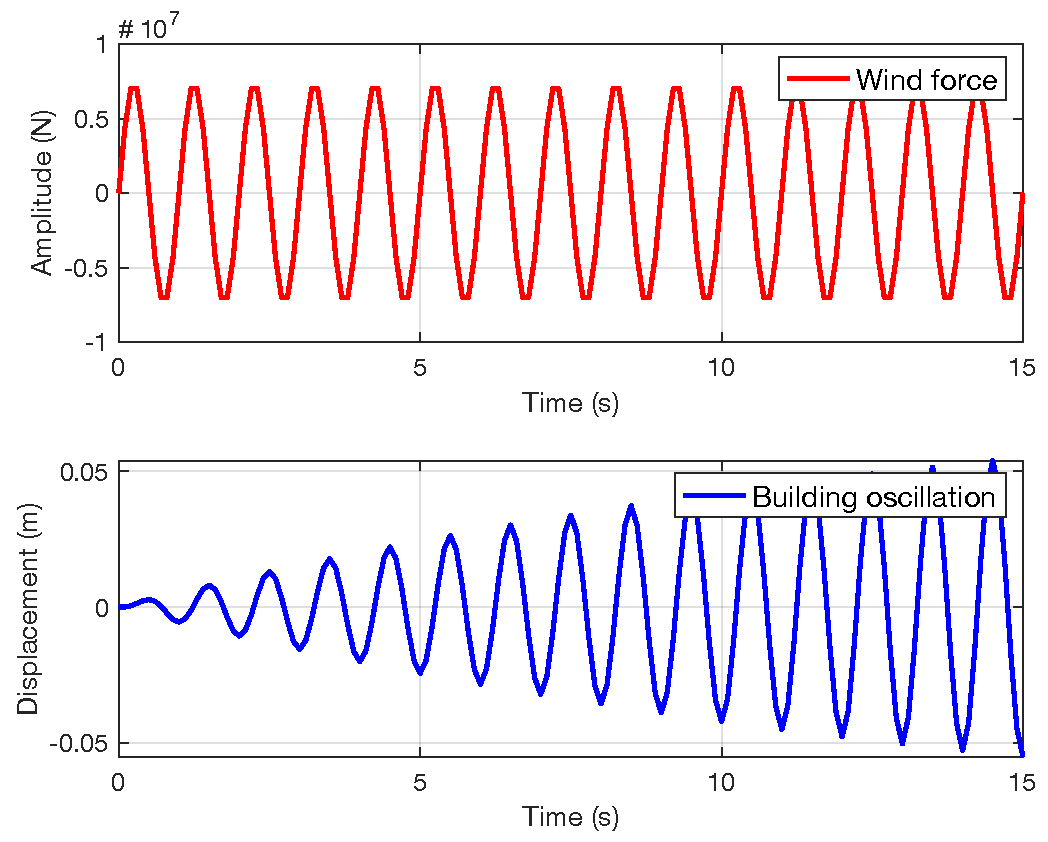
\includegraphics[width=\textwidth]{resources/pdf/sinusoidal.pdf}
        \caption{Sinusoidal wind force}
    \end{subfigure}
    \begin{subfigure}{0.495\textwidth}
        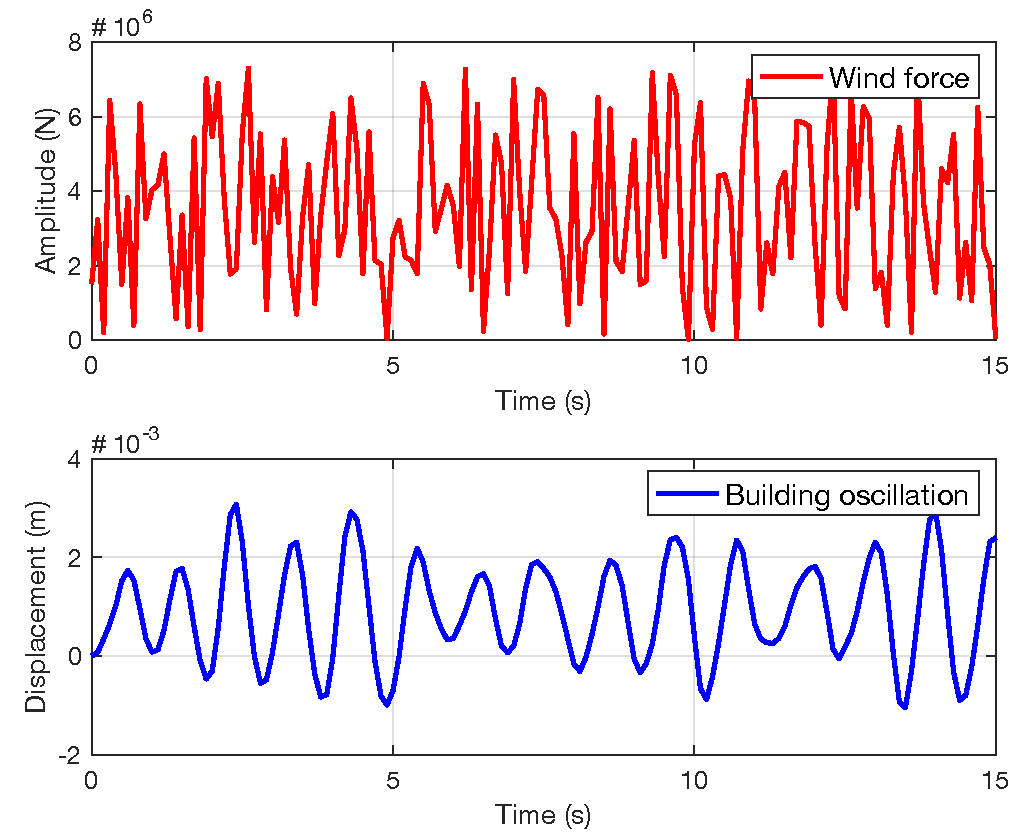
\includegraphics[width=\textwidth]{resources/pdf/random.pdf}
        \caption{Random wind force}
    \end{subfigure}
    \noskipcaption{Simulation results}
\end{figure}
The first simulation (figure \ref{fig:q4.initial}) is a response of our system to initial conditions : the initial displacement of the building is defined at \SI{0.5}{\meter}. We observe that the building oscillates and tends to regain its reference position.\par
The other simulations are responses of our system to an input (the wind).\par
In the case of a constant force (figure \ref{fig:q4.constant}), the building oscillates at the beginning and then tends to stabilize (at a position different from its reference).\par
In cases of sinusoidal and random forces, the building oscillates and follows approximately the wind movement.

    \subsection{State-space representation analysis}

% Stability
\subsubsection{Stability}
To study the stability of the system, we compute the eigenvalues of the dynamic matrix $A$ thanks to Matlab function (\texttt{eig}) :
\begin{align*}
    \lambda_1 &= \num{-5 + 8.6603i}\\
    \lambda_2 &= \num{-5 - 8.6603i}\\
    \lambda_3 &= \num{-0.0628 + 6.2828i}\\
    \lambda_4 &= \num{-0.0628 - 6.2828i}
\end{align*}
The system is stable if the real parts of the eigenvalue are all negative. In our case, the system is stable.

% Observability
\subsubsection{Observability}
To determine whether or not the system is observable, we compute the observability matrix thanks to Matlab function (\texttt{obsv}).\par
The matrix is full rank (verified with Matlab), the system is thus fully observable.\par
As seen on the matrix C, we need one sensor. According to the place of the non zero value, this sensor has to measure the $x_1$ state, namely the horizontal position of the top of the building $d_1$. This state is indeed the objective of the active mass damper and has thus to be observed.

% Controllability
\subsubsection{Controllability}
To determine whether or not the system is controllable, we compute the controllable matrix thanks to Matlab function (\texttt{ctrb}). In order not to take into account the uncontrollable input (wind), only the second column of the B matrix was kept for the calculation.\par
The matrix is full rank (verified with Matlab), the system is thus fully controllable.\par
As seen on matrix B, we need only one actuator. The first column of the $B$ matrix represents the wind, while the second one concerns the damper. This latter is indeed the only controllable input and contains two non-zero elements. As a result, only one actuator is needed, and acts on two states, the speed of the building and the speed of the damper, as they take place on $x_2$ and $x_4$.

    
    % ----- Homework 3 : Controller in time domain ----- %
    \section{Controller in time domain}
    \subsection{State feedback controller}
As the reference is 0, we need not care about $k_r$, so we can fix it to 0.\par
However, if the reference was to change, we could compute $k_r$, it would be nice. Some tests of a change in reference will be performed in this report.\par
In a first time, we only need to compute the gain matrix $K$.\par
In order not to apply a gain on the wind force, our matrix K is as follows :
$$
K = \begin{pmatrix}
    0 & 0 & 0 & 0\\ 
    g_1 & g_2 & g_3 & g_4
\end{pmatrix}
$$
The new dynamic matrix of the closed-loop system is $A_{CL} = A - BK$. Let's determine the eigenvalues of that matrix.\par
As we have a matrix of dimension $4$, we will make the approximation of the dominant poles. Indeed, we have, from the previous matrix $A$, the eigenvalues :
\begin{align*}
    \lambda_1 &= \num{-5 + 8.6603i}\\
    \lambda_2 &= \num{-5 - 8.6603i}\\
    \lambda_3 &= \num{-0.0628 + 6.2828i}\\
    \lambda_4 &= \num{-0.0628 - 6.2828i}
\end{align*}
We can see that $\lambda_1$ and $\lambda_2$ are about $100$ times bigger than the last two, and so we do not need to work on them. Those two will therefore remain in $A_{CL}$.\par
Imposing that $(s - \lambda_1)(s - \lambda_2)$ is part of the decomposition, we get that the determinant of $A_{CL}$ is equal to :
$$
(s - \lambda_1)(s - \lambda_2)(s^2 + 2 \xi\omega_c s + \omega_c^2) = 0
$$
Since $\lambda_1$ and $\lambda_2$ are fixed, we only need to solve the equation of the second degree in $s$ in order to find the expressions of $\lambda_3$ and $\lambda_4$ as a function of $\xi$ and $\omega_c$.\par
The solutions of the equation are given by :
$$
\begin{cases}
    \lambda_3 = -\xi\omega_c - \omega_c\sqrt{\xi^2 - 1}\\
    \lambda_4 = -\xi\omega_c + \omega_c\sqrt{\xi^2 - 1}
\end{cases}
$$
The values of $\xi$ and $\omega_c$ will be determined by simulations in the following sections. When these have been fixed, we will obtain the values of the 4 poles of $A_{CL}$. Then we will just have to use the \texttt{place} function of Matlab to obtain the values $g_i$ of matrix $K$ associated with the eigenvalues.

    \subsection{Observer}
We need to compute the gain matrix $L$ :
$$
L = \begin{pmatrix}
    l_1\\
    l_2\\
    l_3\\
    l_4
\end{pmatrix}
$$
The new dynamic matrix is given by $A_{obs} = A - LC$.\par
As previously, we will keep the same two dominant eigenvalues and determine the two other via the same method we have used for $K$.\par
Imposing that $(s - \lambda_1)(s - \lambda_2)$ is part of the decomposition, we get that the determinant of $A_{obs}$ is equal to :
$$
(s - \lambda_1)(s - \lambda_2)(s^2 + 2 \xi\omega_c s + \omega_c^2) = 0
$$
Since $\lambda_1$ and $\lambda_2$ are fixed, we only need to solve the equation of the second degree in $s$ in order to find the expressions of $\lambda_3$ and $\lambda_4$ as a function of $\xi$ and $\omega_c$.\par
The solutions of the equation are given by :
$$
\begin{cases}
    \lambda_3 = -\xi\omega_c - \omega_c\sqrt{\xi^2 - 1}\\
    \lambda_4 = -\xi\omega_c + \omega_c\sqrt{\xi^2 - 1}
\end{cases}
$$
As for the $K$ matrix, the values of $\xi$ and $\omega_c$ will be determined by simulations in the following sections. When these have been fixed, we will obtain the values of the 4 poles of $A_{obs}$ and will use the \texttt{place} function of Matlab to obtain the values $l_i$ of matrix $L$ associated with the eigenvalues.

    \subsection{Constraints and simulations specifications}
The numerical values used for the simulations are identical to those used previously (homework 2).\par
The reference is set at $0$. It could possibly vary, but by a few centimetres at most.\par
The uncontrolled input signal is the wind. Its values have been determined previously (homework 2). The controlled input signal is the force applied to the damper mass to set it in motion. This force is between \num{0} and \SI{0}{\newton}.\par
The system consists of 4 states. The output is one of the states. In order to ensure that the behaviour of the system is physically realistic, we set a value domain for each state and will check in the simulations whether the values obtained belong to these domains.
\begin{table}[H]
    \centering
    \begin{tabular}{|l|c|}
        \hline
        {\bf State} & {\bf Domain}\\ \hline
        \hline
        $x_1 = d_1$ & ...\\ \hline
        $x_2 = \dot{d}_1$ & ...\\ \hline
        $x_3 = d_2$ & ...\\ \hline
        $x_4 = \dot{d}_2$ & ...\\ \hline
    \end{tabular}
    \caption{Range of acceptable values for each state}
\end{table}

    \subsection{System simulations without controller}
To simulate the system (without control mechanism), we choose a series of numerical values, presented in table \ref{tab:numerical_values}\footnote{We would like to thank Professor Denoël for discussing these values with us.}.
\begin{table}[H]
    \centering
    \begin{tabular}{|l|c|c|}
        \hline
        {\bf Mass} & $m_1 = \SI{1e8}{\kilogram}$ & $m_2 = \SI{1e3}{\kilogram}$\\ \hline
        {\bf Spring} & $k_1 \approx \SI{4e9}{\newton/\meter}$ & $k_2 = \SI{e5}{\newton/\meter}$\\ \hline
        {\bf Damper} & $c_1 \approx \SI{1.3e7}{\newton\second/\meter}$ & $c_2 = \SI{e4}{\newton\second/\meter}$\\ \hline
        {\bf Wind} & \multicolumn{2}{c|}{$F_{max} = \SI{7.35e6}{\newton}$}\\ \hline
    \end{tabular}
    \caption{Numerical values of the system}
    \label{tab:numerical_values}
\end{table}
For the strength of the wind, we considered 2 cases (in newton) :
\begin{align*}
    F_1 &= F_{max}\quad\forall t & \text{Constant wind force}\\
    F_1(t) &= F_{max}\sin(2\pi t) & \text{Sinusoidal wind force}
\end{align*}
The stiffness and viscosity values for the building were obtained using the formulas :
\begin{align*}
    k_1 &= (2\pi f)^2m_1\\
    c_1 &= 2m_1(2\pi f)0.01
\end{align*}
where $f = \SI{1}{\hertz}$ is the natural frequency associated with the mass of the building.\par
The maximum wind force, on the other hand, was approximated by
\begin{equation*}
    F_{max} = \frac{1}{2}\rho v^2A
\end{equation*}
with
\begin{itemize}
    \item $\rho \approx \SI{1.2}{\kilogram/\meter\cubed}$, the air density;
    \item $v = \SI{35}{\meter/\second}$, the wind speed;
    \item $A = 250\times 40 = \SI{10000}{\meter\squared}$, the area of one side of the building.
\end{itemize}
\subsubsection{Simulation results}
\begin{figure}[H]
    \centering
    \begin{subfigure}{0.495\textwidth}
        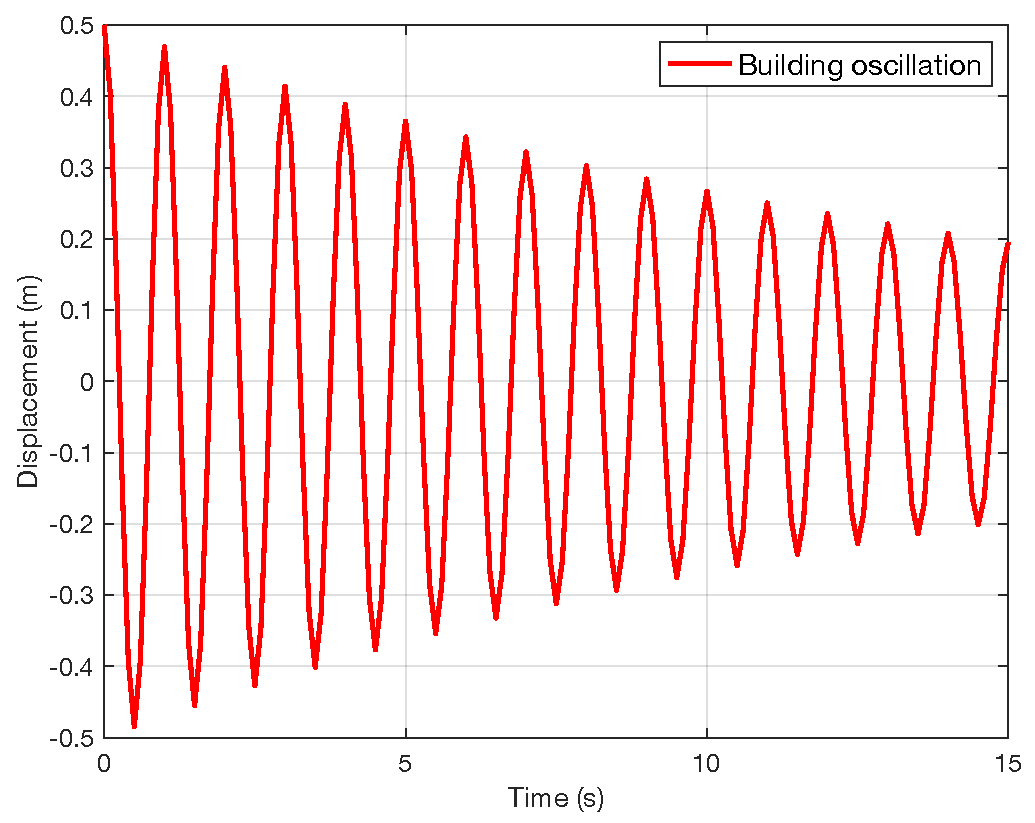
\includegraphics[width=\textwidth]{resources/pdf/initial.pdf}
        \caption{Initial conditions}
        \label{fig:q4.initial}
    \end{subfigure}
    \begin{subfigure}{0.495\textwidth}
        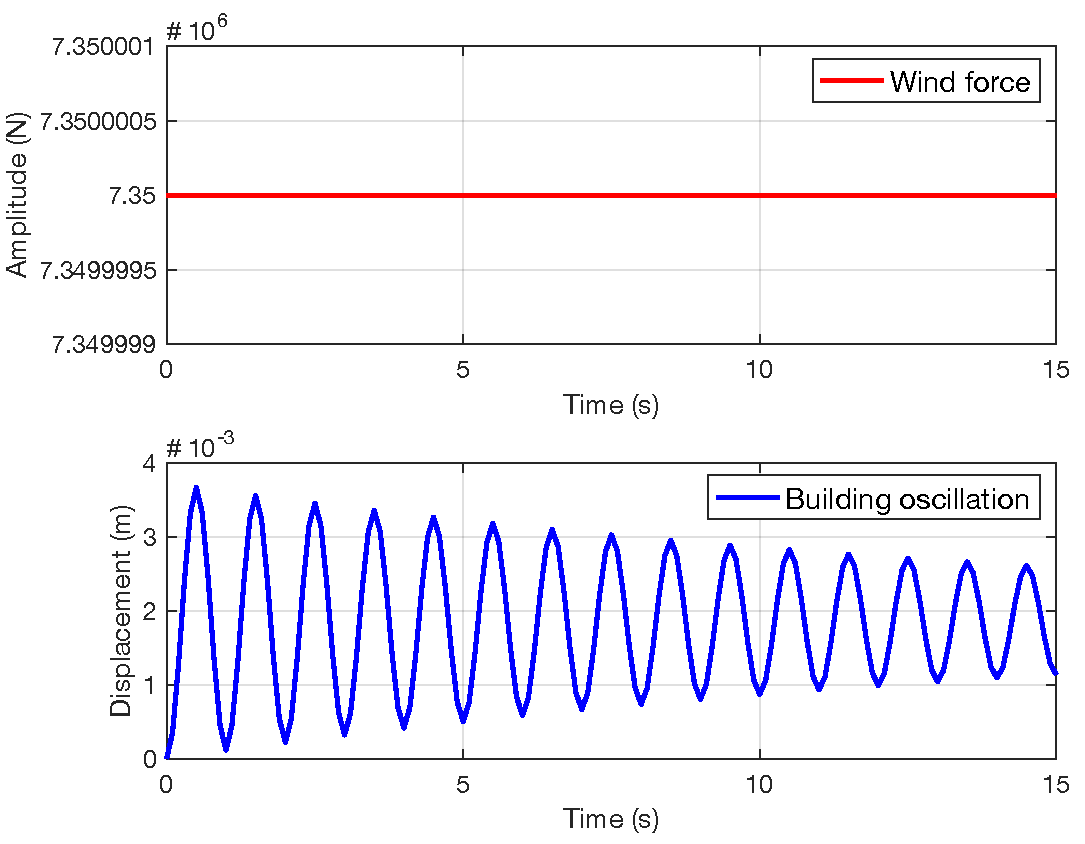
\includegraphics[width=\textwidth]{resources/pdf/constant.pdf}
        \caption{Constant wind force}
        \label{fig:q4.constant}
    \end{subfigure}
    \begin{subfigure}{0.495\textwidth}
        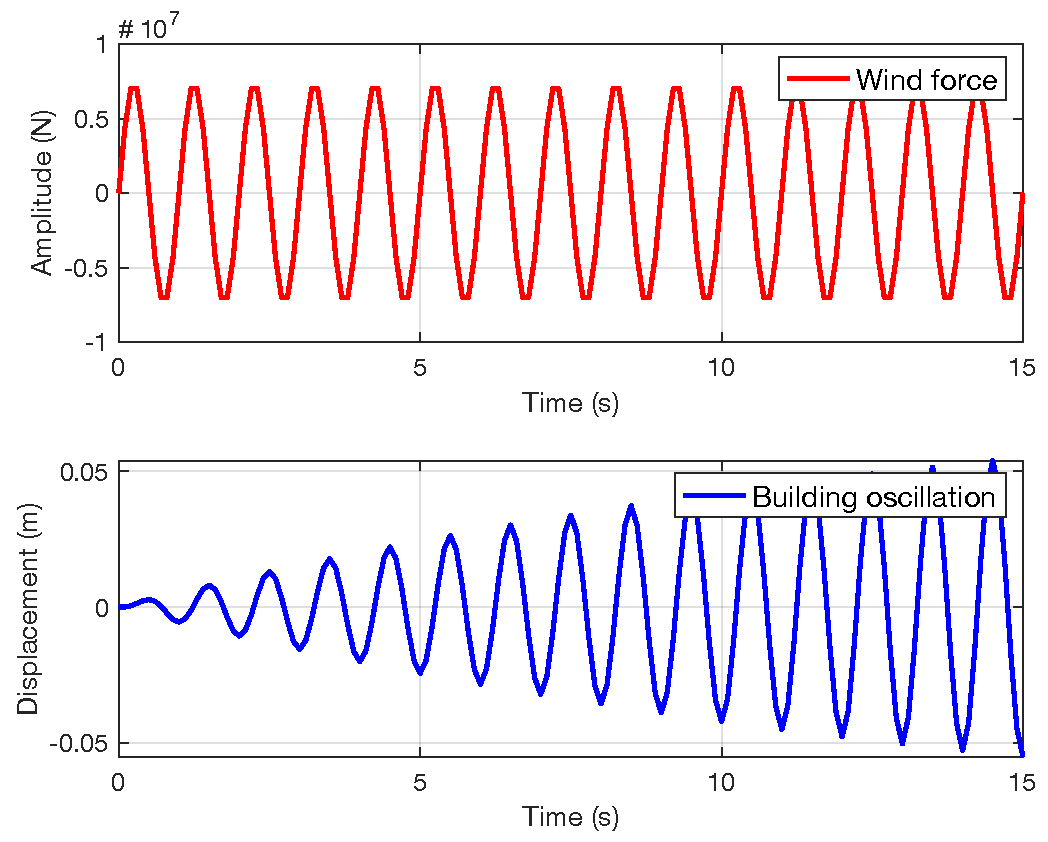
\includegraphics[width=\textwidth]{resources/pdf/sinusoidal.pdf}
        \caption{Sinusoidal wind force}
    \end{subfigure}
    \begin{subfigure}{0.495\textwidth}
        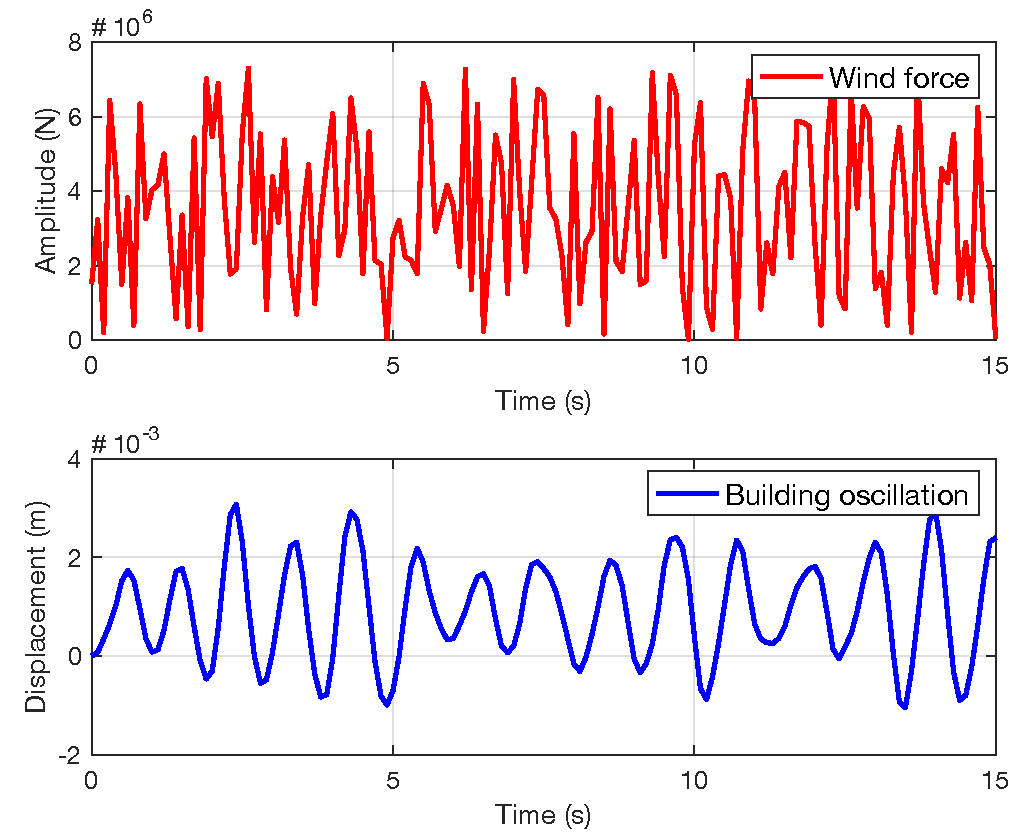
\includegraphics[width=\textwidth]{resources/pdf/random.pdf}
        \caption{Random wind force}
    \end{subfigure}
    \noskipcaption{Simulation results}
\end{figure}
The first simulation (figure \ref{fig:q4.initial}) is a response of our system to initial conditions : the initial displacement of the building is defined at \SI{0.5}{\meter}. We observe that the building oscillates and tends to regain its reference position.\par
The other simulations are responses of our system to an input (the wind).\par
In the case of a constant force (figure \ref{fig:q4.constant}), the building oscillates at the beginning and then tends to stabilize (at a position different from its reference).\par
In cases of sinusoidal and random forces, the building oscillates and follows approximately the wind movement.

    
    % ----- Homework 4 : Frequency domain ----- %
    \section{Frequency domain}
    \subsection{Constraints and simulation specifications}
We have the following constraints : 
\begin{itemize}
    \item Acceleration of the mass damper between \num{0.3} and \num{0.6}$g$, as advised by Prof. Denoël.
    \item Power injected in the mass of below \SI{10}{\kilo\watt} so as to not have too much electrical consumption.
    \item Lateral movement of the top of the building not above \SI{1}{\meter}.
\end{itemize}
The scenario we look at is the following : 
A turbulent wind of maximum \SI{7.35}{\mega\newton}, that we represented as a sine function.
\subsubsection{Choice of cross-over frequency}
The frequency of our damper is computed via : $f = \sqrt{\dfrac{k}{m}} \approx \SI{10}{\hertz}$. We will therefore use a crossover frequency of \SI{20}{\hertz}, so all frequencies above that, probably coming from noise and unwanted phenomena, will be attenuated, while the amplitudes of the frequencies below that, which correspond to the internals of our system, will be amplified.

    \subsection{Loop shaping}
to do

    \subsection{Gang of four}
to do

    \subsection{Delays through the controller design}
to do

    
    % ----- References ----- %
    \newpage
    \subsection{References}
    \nocite{*}
    \printbibliography
\end{document}
